\documentclass[12pt]{report}
\usepackage{xcolor}
\usepackage{titlesec}
\usepackage{graphicx}
\usepackage{pgffor}
\usepackage{subcaption}
\usepackage{etoolbox}
\usepackage{pgfkeys, pgfplots, filecontents}
\usepackage{filecontents}

% Define colors for chapter and section titles
\definecolor{blue}{rgb}{0.0, 0.0, 1.0}
\definecolor{red}{rgb}{1.0, 0.0, 0.0}

% Customize chapter and section formatting
\titleformat{\chapter}[hang]{\normalfont\Large\bfseries\color{blue}}{\thechapter}{1em}{}[\titlerule]
\titleformat{\section}[hang]{\normalfont\large\bfseries\color{red}}{\thesection}{1em}{}

\begin{document}
\title{Machine Visual Perception\\Course Project Report}
\author{Authors: Mario Pariona, Leo Takashige, Kee Yun Shao\\ Group number: 9}
\date{\today}
\maketitle

\chapter{Introduction and Motivation}
\section{Introduction to the problem}
Meshes and points are the most common 3D scene representations. However, although easily parallelizable, they are not differentiable. This limitation poses significant challenges for tasks that require gradient-based optimization, such as neural rendering and scene reconstruction.

\section{Background and related work}
Traditional scene reconstruction and rendering techniques have relied heavily on mesh-based representations. While effective, these methods often struggle with complex scenes and require extensive manual effort to achieve high-quality results.

Neural rendering and radiance fields have emerged as powerful alternatives, leveraging neural networks to model the appearance and geometry of 3D scenes. These methods have demonstrated impressive results in generating photorealistic images and enabling novel view synthesis.

Point-based rendering and radiance fields offer another promising approach, combining the simplicity of point clouds with the flexibility of neural networks. This hybrid method aims to overcome the limitations of traditional mesh-based techniques while maintaining the benefits of differentiability and scalability.

\section{Overview of the idea}
The famous paper “3D Gaussian Splatting for Real-Time Radiance Field Rendering” presents the idea of using 3D Gaussians to model a scene. However, in its simplest form, the number of Gaussians won’t change, or it would only decrease over time. Therefore, it presents the idea of Adaptive Density Control. This suggests that every 100 iterations, it will first delete the Gaussians whose transparency $\alpha$ is less than a threshold $\epsilon_\alpha$.
Then, it will add new Gaussians to the scene based on the density of the existing ones. This adaptive approach allows the model to dynamically adjust the number of Gaussians, improving the representation of the scene over time. The process ensures that the Gaussians are distributed more effectively, focusing computational resources on the most important areas of the scene.

\chapter{Method}

\section{Baseline Algorithm}
In this section, we describe the baseline architecture used as the foundation for our algorithm. The baseline is based on the 3D Gaussian Splatting (3D-GS) technique, which models a scene using 3D Gaussians. The original paper presents a method for real-time radiance field rendering using a fixed number of Gaussians. Figures from the original paper are reproduced here to illustrate the baseline architecture.

\section{Algorithm Improvements}
To improve upon the baseline, we implemented several enhancements. The key improvement is the introduction of Adaptive Density Control, which dynamically adjusts the number of Gaussians in the scene. Every 100 iterations, Gaussians with transparency $\alpha$ below a threshold $\epsilon_\alpha$ are removed, and new Gaussians are added based on the density of existing ones. This adaptive approach ensures a more efficient and accurate representation of the scene. Figures are included to explain the idea and logic behind these improvements.

\section{Implementation Details}
The improvements were implemented using Python and PyTorch. The adaptive density control mechanism was integrated into the training loop, allowing for dynamic adjustment of Gaussians during training. Below are code snippets illustrating the key parts of the implementation:


\section{Datasets}
We used the well-known Mip-NeRF360 dataset [Mildenhall et al. 2019] and LLFF dataset [Knapitsch et al. 2017] for training and testing our model. Additionally, we created two scenes for our own dataset and used synthetic scenes from the Synthetic Blender dataset. The datasets were preprocessed to extract training and testing images, which were then fed into the model for training and evaluation.

MipNeRF360 outdoor:
\begin{itemize}
    \item Bicycle 
    \item Stump
\end{itemize}

MipNeRF360 Indoor:
\begin{itemize}
    \item Counter (indoor)
\end{itemize}

Deep Blending:
\begin{itemize}
    \item Playroom
\end{itemize}

Tanks and Temples:
\begin{itemize}
    \item Truck
    \item Train
\end{itemize}

LLFF:
\begin{itemize}
    \item Horns (62 images)
    \item T-rex (55 images)
\end{itemize}

Same as NeRF, 3D-GS and the ERM, we take each 8th image for the test set and others for the training set.

\section{Training and testing results}
[Explain the training and testing results with graphs and elaborating on why they make sense, what could be improved.]

\section{Qualitative results}
We test our model on both real-world scenes from previously published datasets, including the Mip-NeRF360 dataset, LLFF dataset, and synthetic scenes from the Deep Blending dataset. The specific scenes used from each dataset are as follows: 

For the MipNeRF360 outdoor dataset, we used the Bicycle and Stump scenes. From the MipNeRF360 indoor dataset, we used the Counter scene. For the Deep Blending dataset, we used the Playroom scene. From the Tanks and Temples dataset, we used the Truck and Train scenes. Lastly, from the LLFF dataset, we used the Horns scene with 62 images and the T-rex scene with 55 images.

[Big picture of as Figure 5 in 3DGS]

\begin{figure}[h]
    \centering
    \begin{tabular}{ccc}
        \textbf{Ground Truth} & \textbf{3D-GS} & \textbf{Ours} \\ \hline
        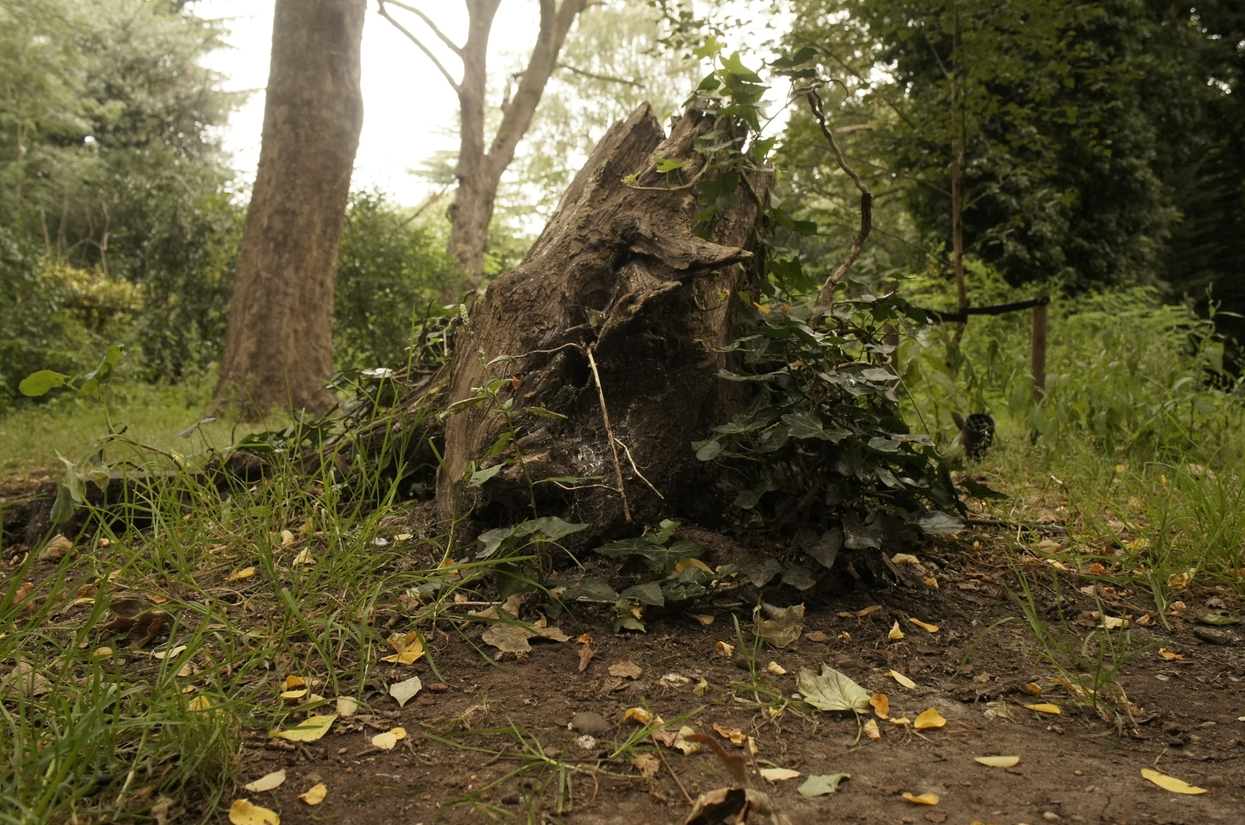
\includegraphics[width=0.3\textwidth]{../o-3dgs/eval/stump/test/ours_30000/gt/00000.png} & 
        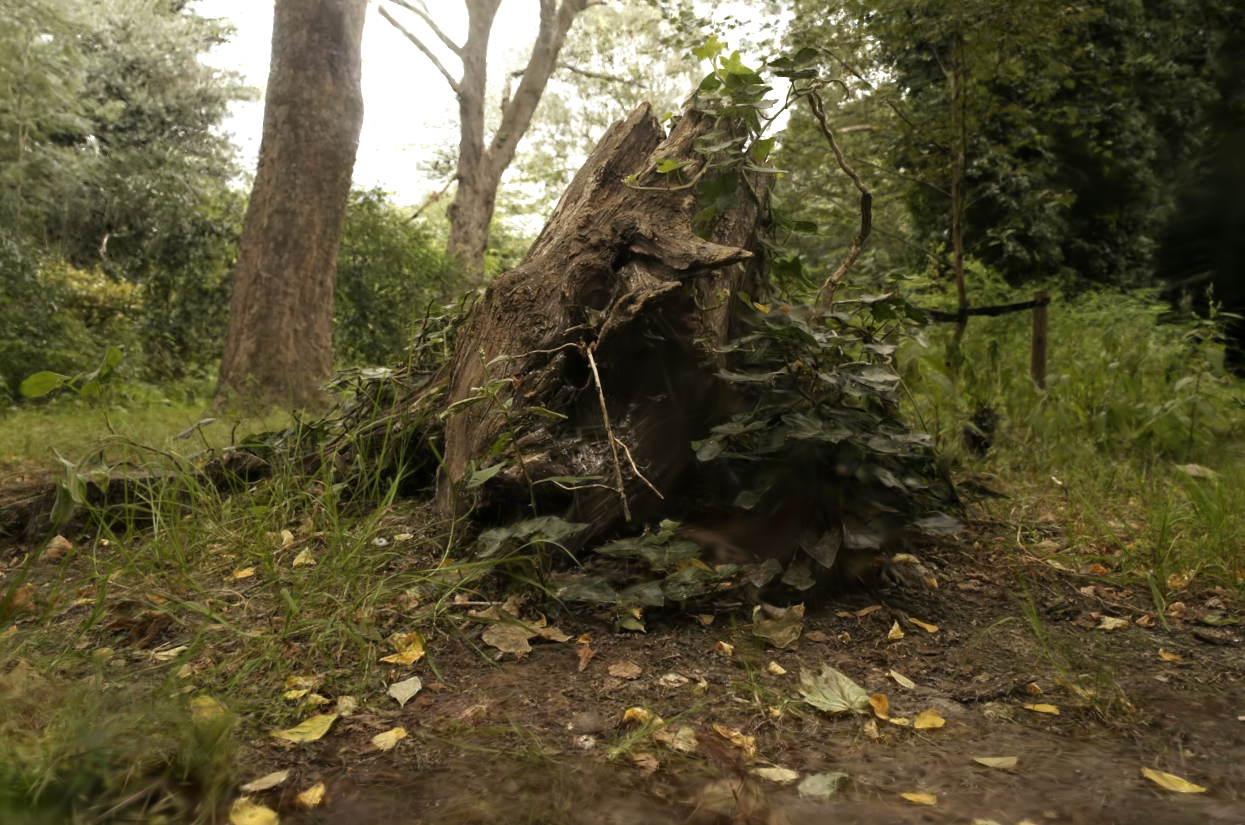
\includegraphics[width=0.3\textwidth]{../o-3dgs/eval/stump/test/ours_30000/renders/00000.png} & 
        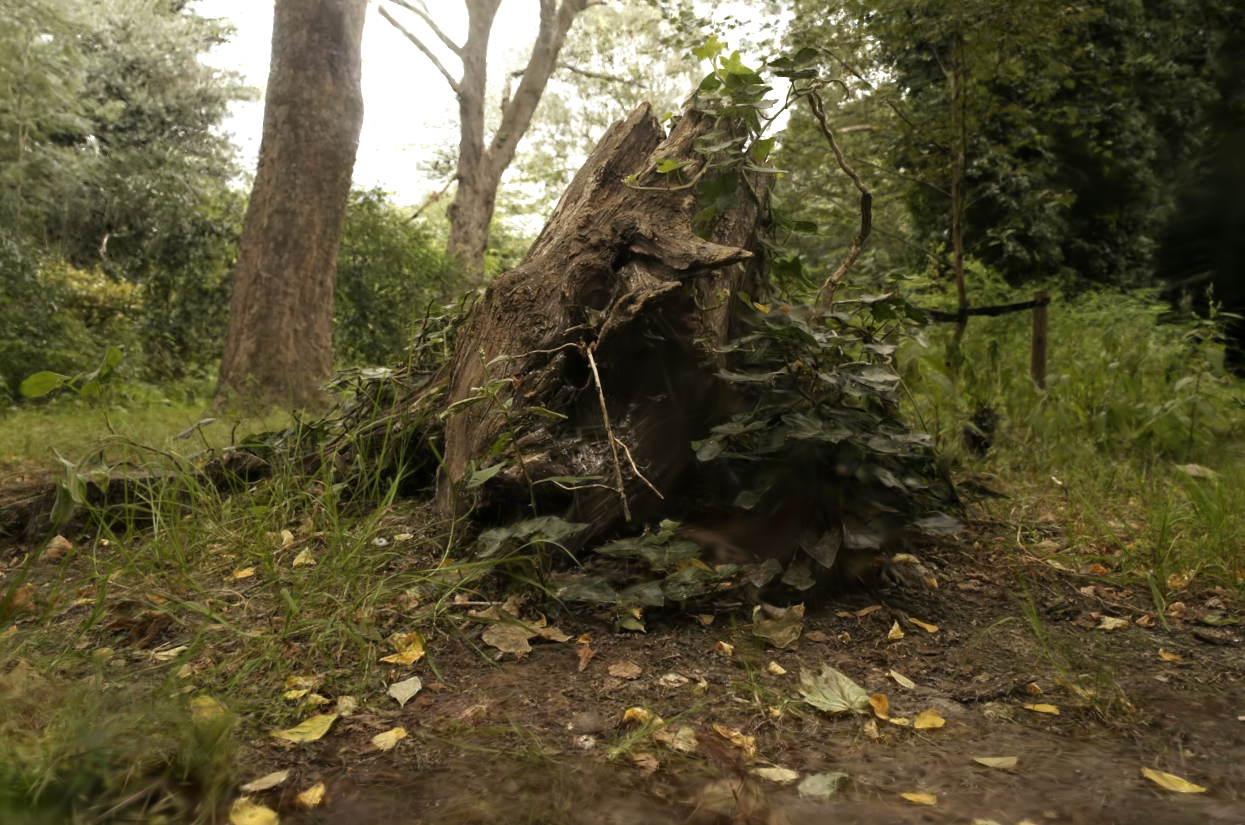
\includegraphics[width=0.3\textwidth]{../o-3dgs/eval/stump/test/ours_30000/renders/00000.png} \\
        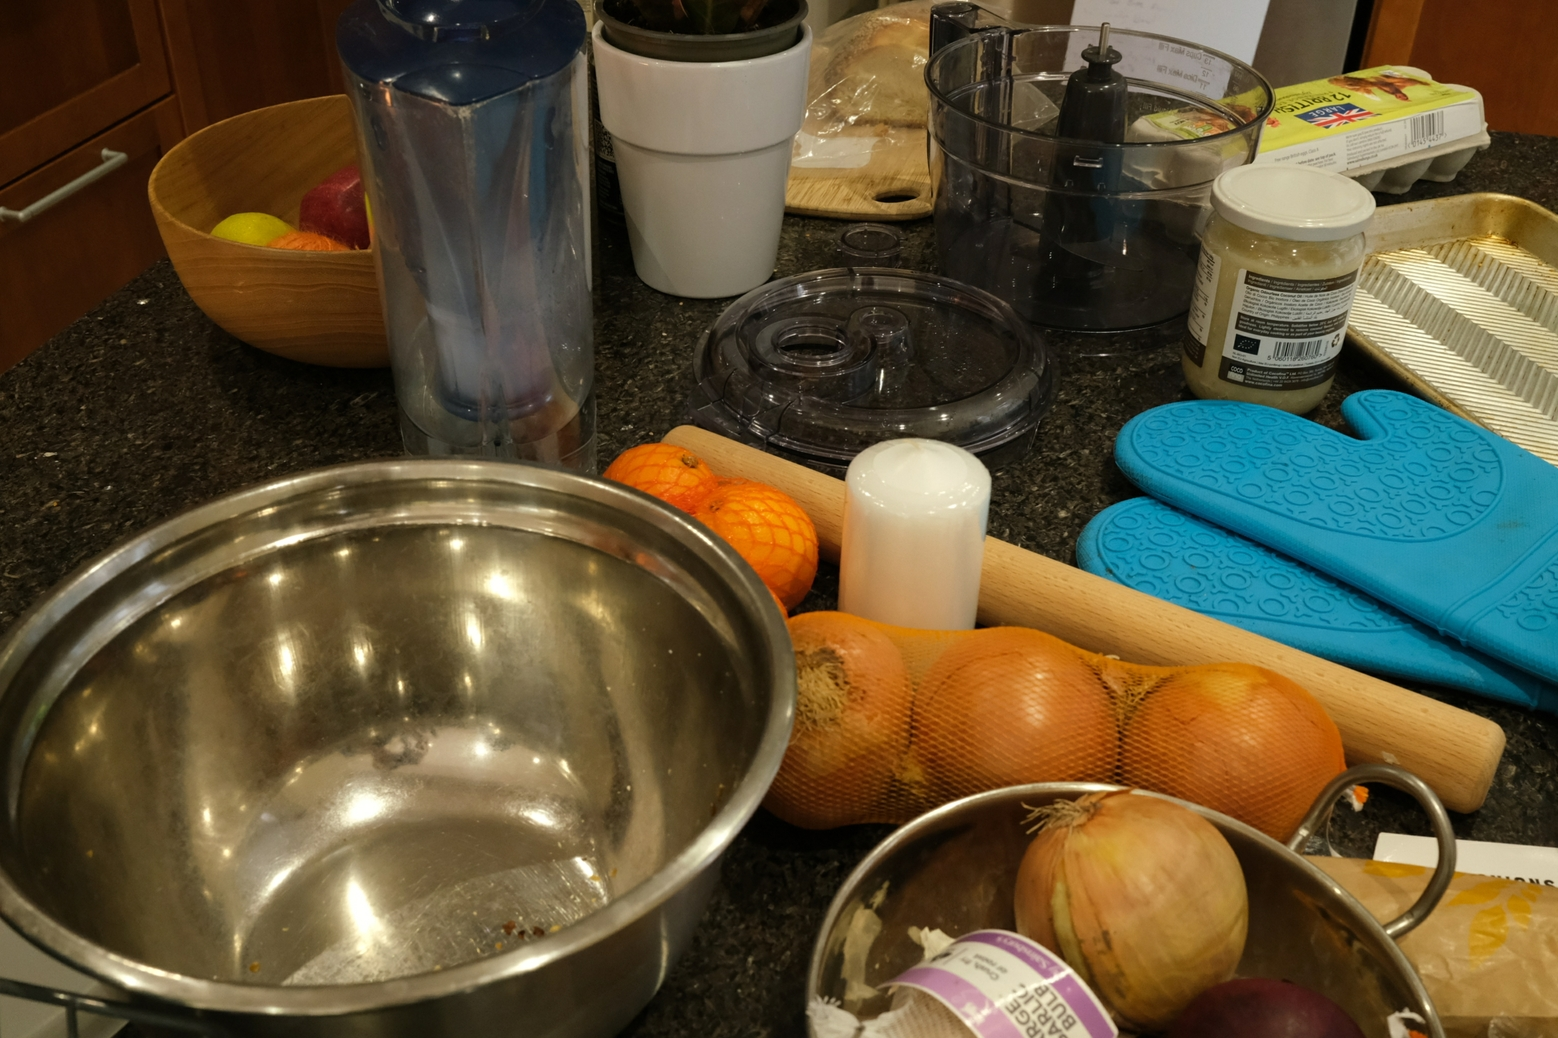
\includegraphics[width=0.3\textwidth]{../o-3dgs/eval/counter/test/ours_30000/gt/00000.png} & 
        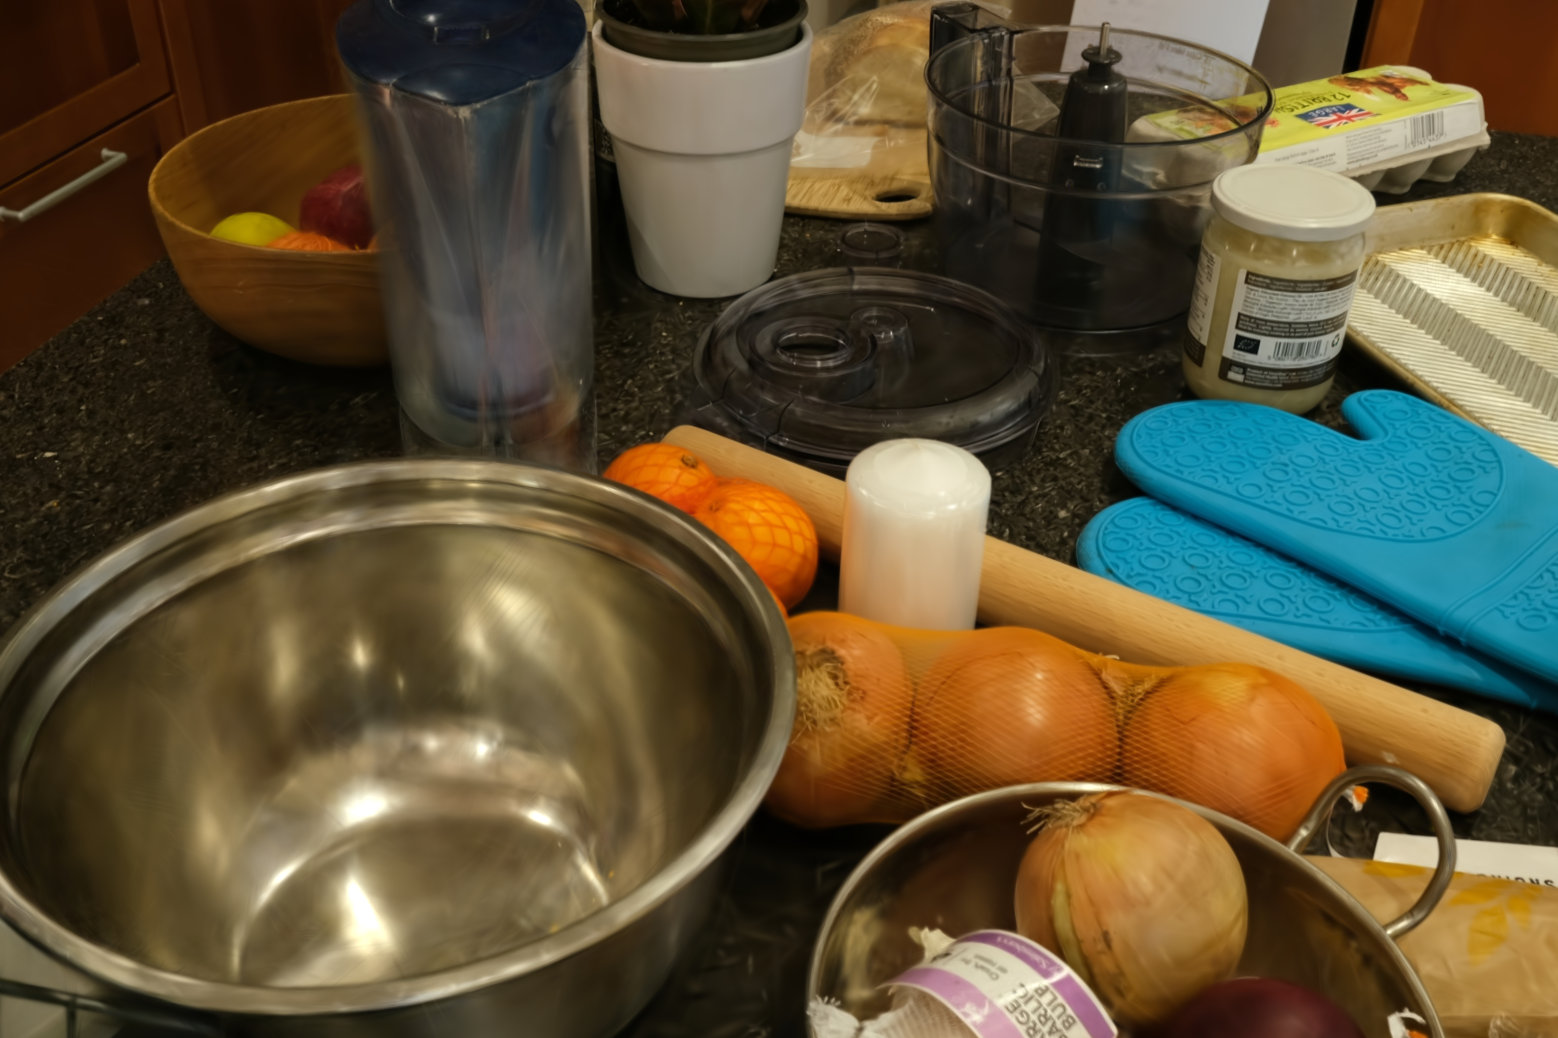
\includegraphics[width=0.3\textwidth]{../o-3dgs/eval/counter/test/ours_30000/renders/00000.png} & 
        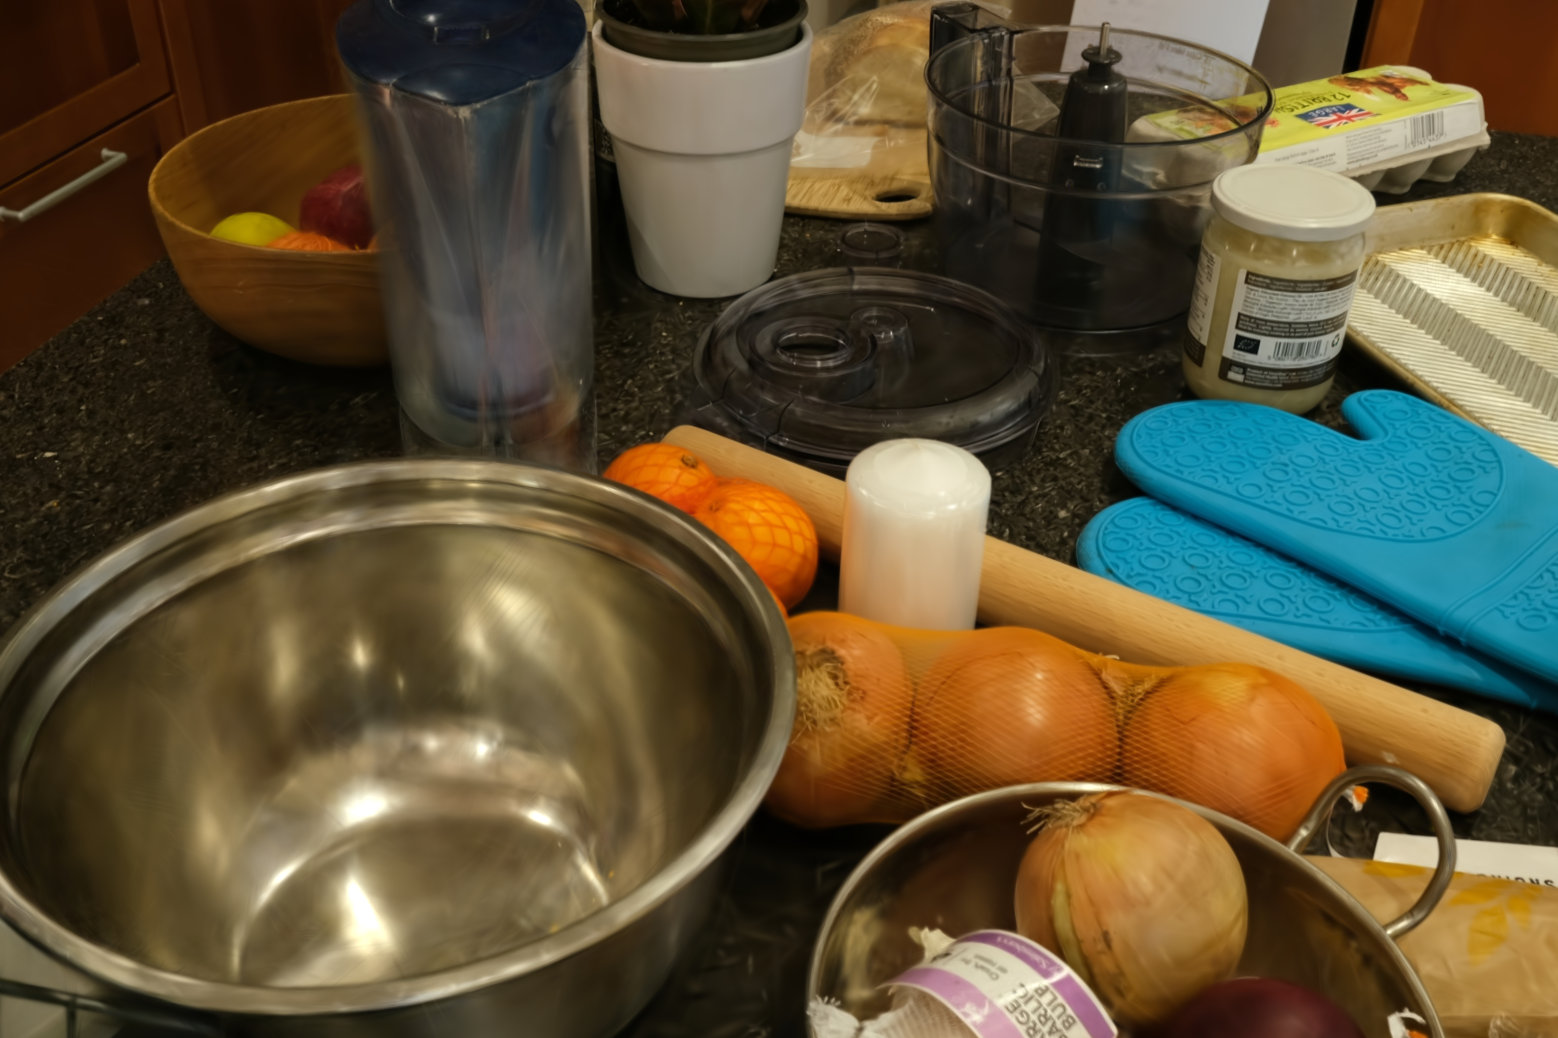
\includegraphics[width=0.3\textwidth]{../o-3dgs/eval/counter/test/ours_30000/renders/00000.png} \\
        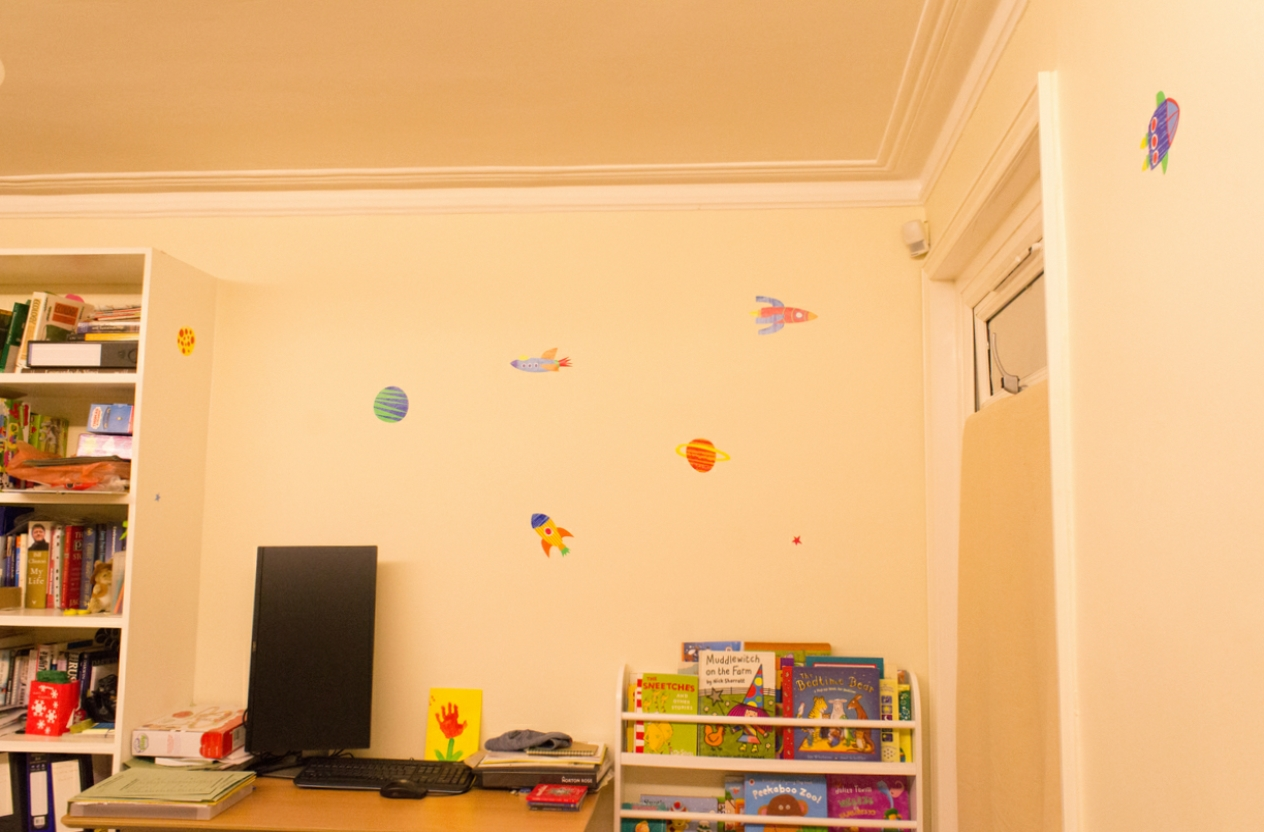
\includegraphics[width=0.3\textwidth]{../o-3dgs/eval/playroom/test/ours_30000/gt/00000.png} & 
        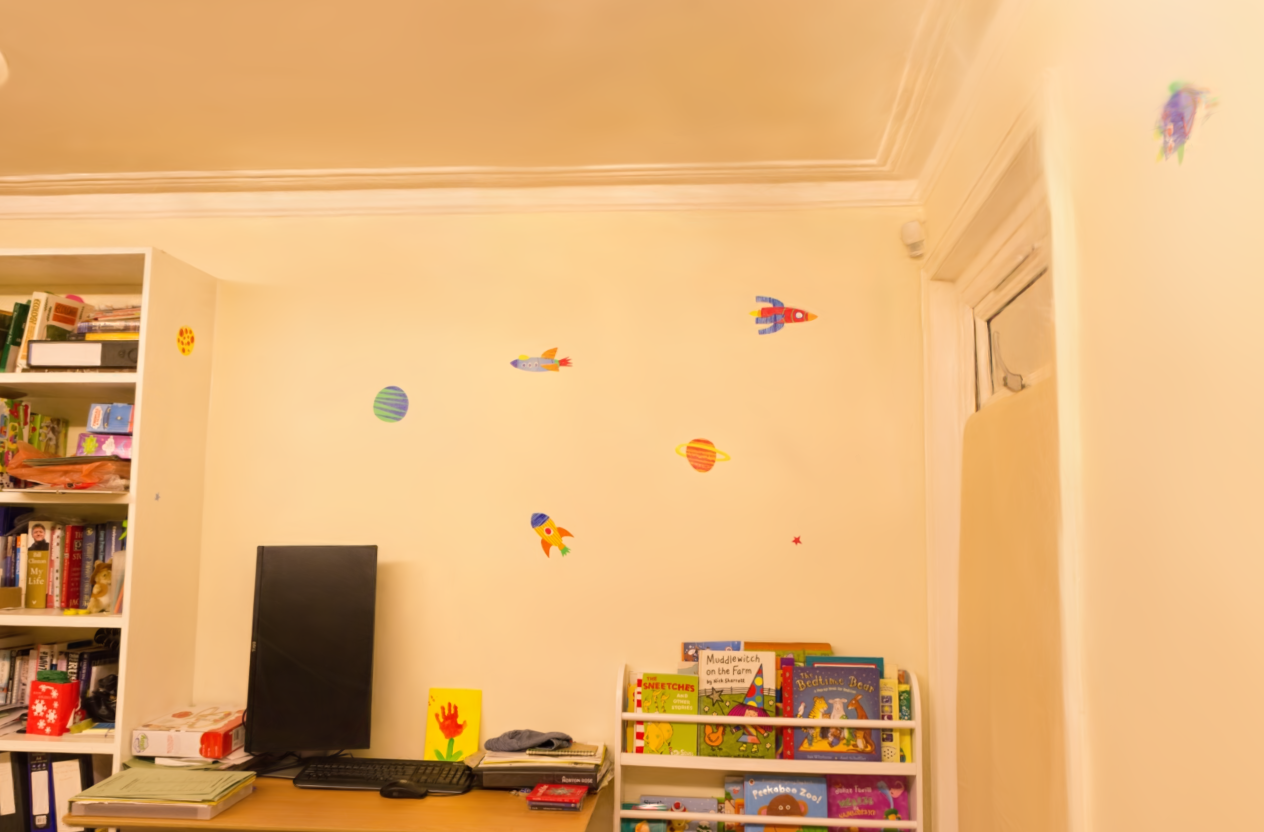
\includegraphics[width=0.3\textwidth]{../o-3dgs/eval/playroom/test/ours_30000/renders/00000.png} & 
        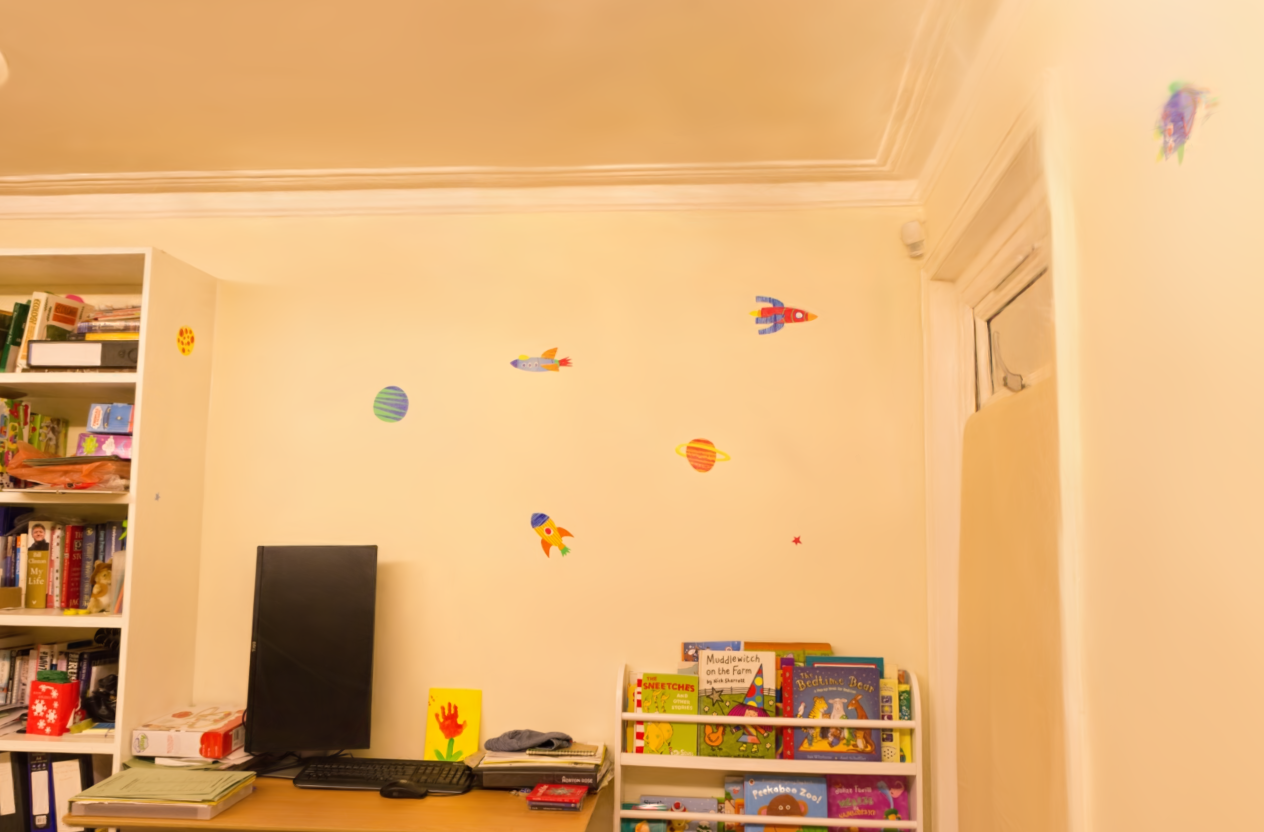
\includegraphics[width=0.3\textwidth]{../o-3dgs/eval/playroom/test/ours_30000/renders/00000.png} \\
        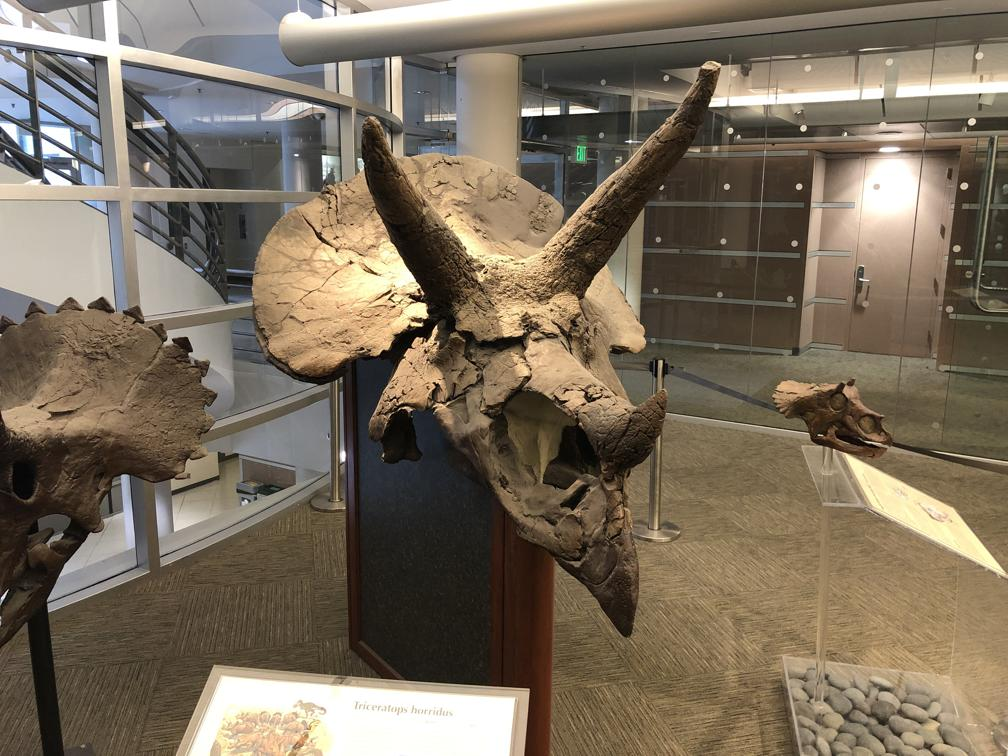
\includegraphics[width=0.3\textwidth]{../o-3dgs/eval/horns/test/ours_30000/gt/00000.png} & 
        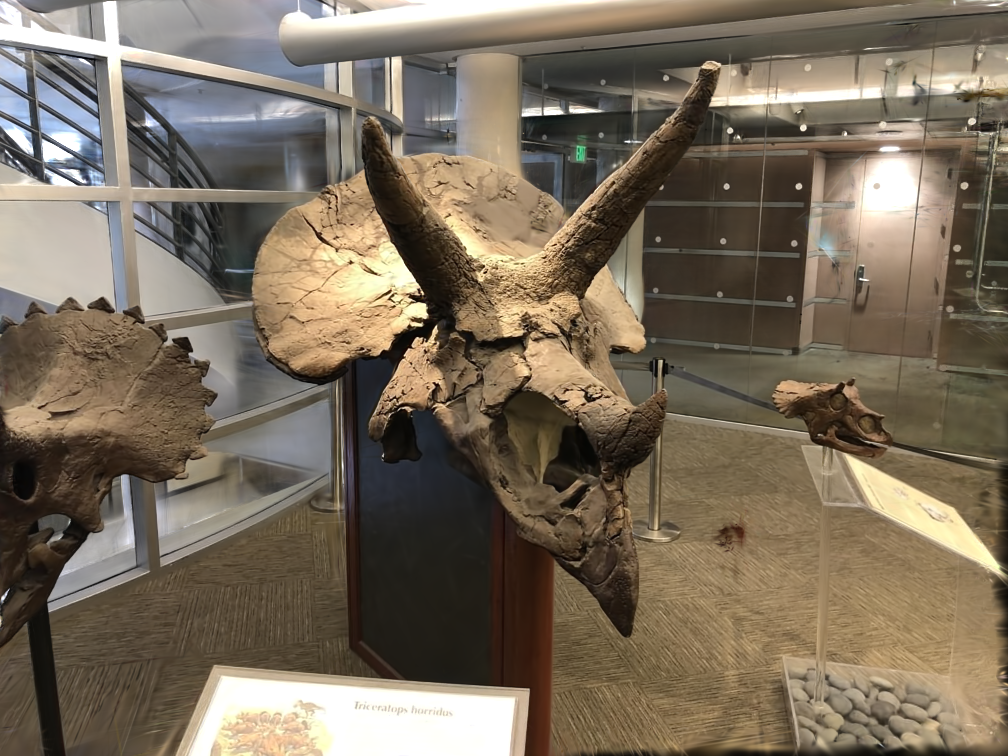
\includegraphics[width=0.3\textwidth]{../o-3dgs/eval/horns/test/ours_30000/renders/00000.png} & 
        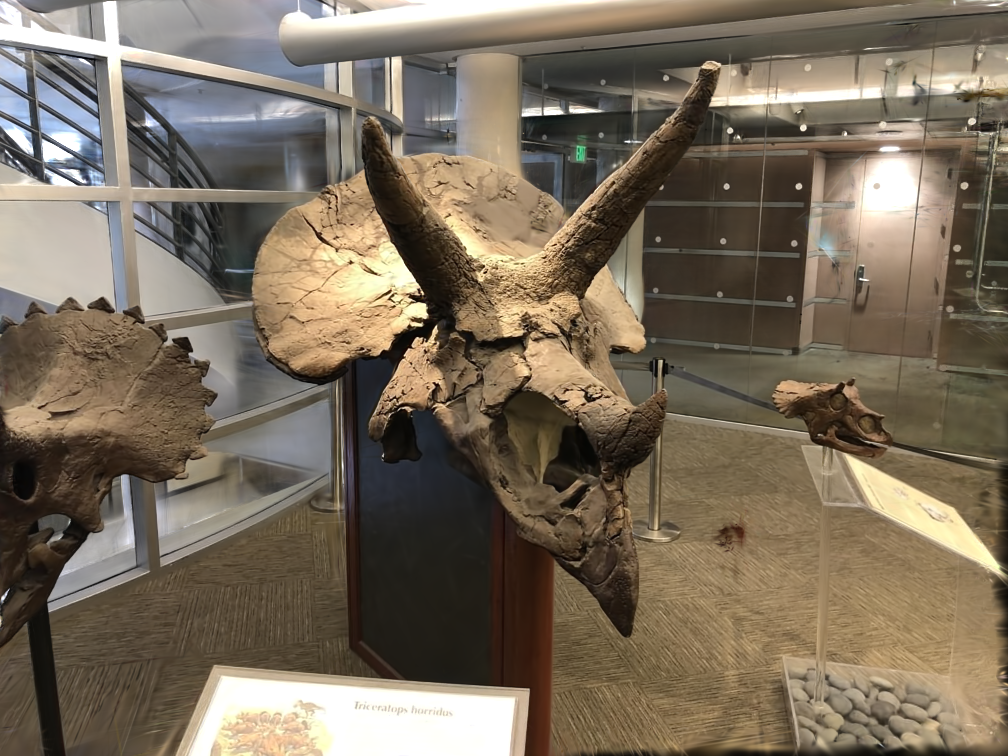
\includegraphics[width=0.3\textwidth]{../o-3dgs/eval/horns/test/ours_30000/renders/00000.png} \\
        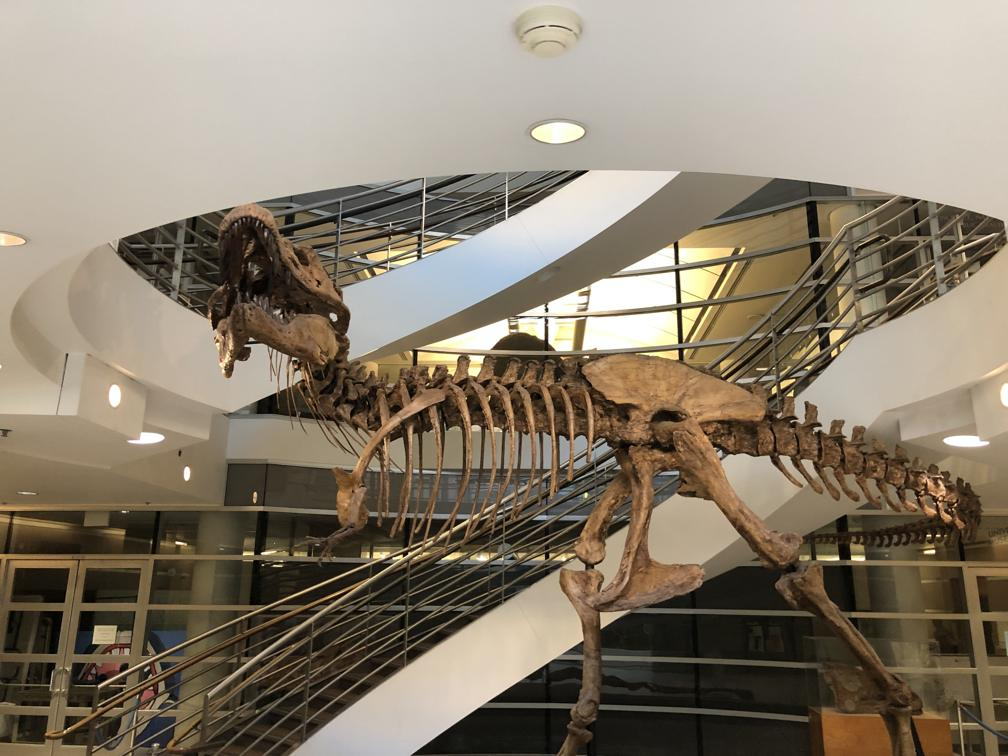
\includegraphics[width=0.3\textwidth]{../o-3dgs/eval/trex/test/ours_30000/gt/00000.png} & 
        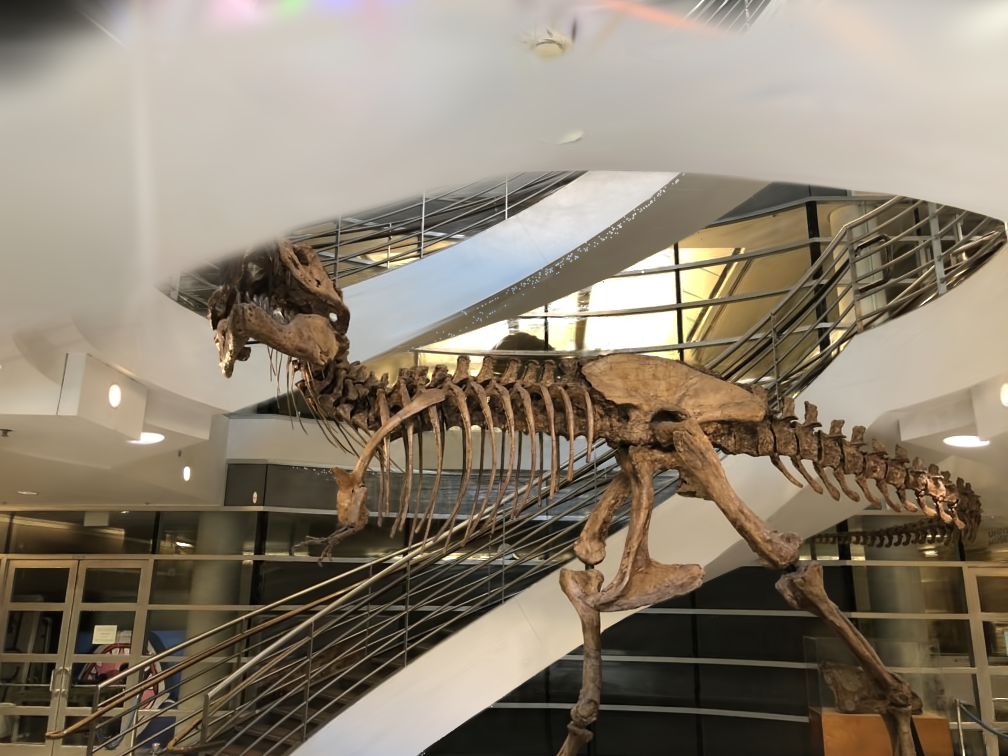
\includegraphics[width=0.3\textwidth]{../o-3dgs/eval/trex/test/ours_30000/renders/00000.png} & 
        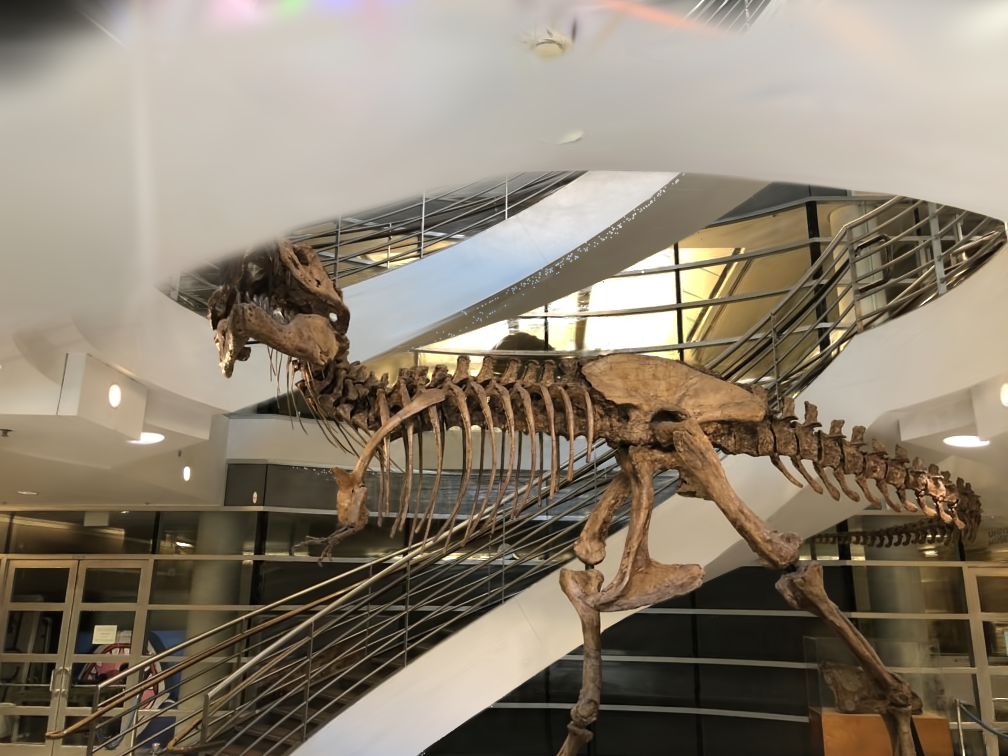
\includegraphics[width=0.3\textwidth]{../o-3dgs/eval/trex/test/ours_30000/renders/00000.png} \\
    \end{tabular}
    \caption{Comparison of Ground Truth, 3D-GS, and Our Results for Different Scenes.}
    \label{fig:comparison_tabular_loop}
\end{figure}
% \begin{figure}[h]
%     \centering
%     \newcommand{\mymatrixcontent}{} % Initialize an empty macro for storing content
    
%     % Loop through the folders
%     \foreach \folder in {stump, counter, playroom, horns, trex} { 
%         \edef\temp{%
%             \noexpand\begin{tabular}{ccc}
%                 \textbf{Ground Truth} & \textbf{3D-GS} & \textbf{Ours} \\ \hline
%                 \noexpand\includegraphics[width=0.3\textwidth]{../o-3dgs/eval/\folder/test/ours_30000/gt/00000.png} & 
%                 \noexpand\includegraphics[width=0.3\textwidth]{../o-3dgs/eval/\folder/test/ours_30000/renders/00000.png} & 
%                 \noexpand\includegraphics[width=0.3\textwidth]{../o-3dgs/eval/\folder/test/ours_30000/renders/00000.png} 
%             \noexpand\end{tabular}
%         }
%         % Append the row content
%         \expandafter\gappto\expandafter{\mymatrixcontent}\expandafter{\temp} 
%     }
    
%     % Now use the accumulated content in the tabular environment
%     \mymatrixcontent % Expanding the accumulated content here

%     \caption{Comparison of Ground Truth, 3D-GS, and Our Results for Different Scenes.}
%     \label{fig:comparison_tabular_loop}
% \end{figure}

    % \foreach \folder in {stump, counter, playroom, horns, trex} { % Replace with actual folder names
    % % \foreach \folder in {bicycle, stump, counter, truck, train, playroom, horns, trex} { % Replace with actual folder names
    %     \begin{subfigure}[b]{0.3\textwidth}
    %         \includegraphics[width=\textwidth]{../o-3dgs/eval/\folder/test/ours_30000/gt/00000.png}
    %         % \caption*{Ground Truth (\folder)}
    %     \end{subfigure}
    %     % \hfill
    %     \begin{subfigure}[b]{0.3\textwidth}
    %         \includegraphics[width=\textwidth]{../o-3dgs/eval/\folder/test/ours_30000/renders/00000.png}
    %         % \caption*{Rendered Image (\folder)}
    %     \end{subfigure}
    %     % \hfill
    %     \begin{subfigure}[b]{0.3\textwidth}
    %         \includegraphics[width=\textwidth]{../o-3dgs/eval/\folder/test/ours_30000/renders/00000.png}
    %         % \caption*{Our Image (\folder)}
    %     \end{subfigure}
        % \vspace{0.5cm} % Space between rows of figures
    % % }
    % \caption{Comparison between Ground Truth, Rendered Images, and Our Images for Different Scenes.}
    % \label{fig:comparison_all}
% \end{figure}

[Could add all the pictures of 3GDS of why everything is needed]

[Ablations, Picture of comparison
 No cloning learnable
No splitting learnable]

\section{Quantitative results}
In this section, we present the quantitative results of our experiments. The performance of our model is evaluated using standard metrics such as PSNR (Peak Signal-to-Noise Ratio), SSIM (Structural Similarity Index), and LPIPS (Learned Perceptual Image Patch Similarity). The results are compared against the baseline 3D-GS method.

\pgfplotsset{compat=1.17}

% \foreach \folder in {bicycle}{
%     from ../o-3dgs/eval/\folder/results.json as x get x["ours_30000"]["PSNR"]
% }

% \pgfkeys{
%     /results/.is family, /results,
%     scene/.initial=,
%     psnr/.initial=,
%     ssim/.initial=,
%     lpips/.initial=
% }

% \newcommand{\readjson}[1]{%
%     \foreach \i in {0,...,4} {%
%         \pgfplotstableread{results.json}\loadeddata
%         \pgfplotstablegetelem{\i}{[index]0}\of\loadeddata
%         \pgfkeyssetvalue{/results/scene}{\pgfplotsretval}
%         \pgfplotstablegetelem{\i}{[index]1}\of\loadeddata
%         \pgfkeyssetvalue{/results/psnr}{\pgfplotsretval}
%         \pgfplotstablegetelem{\i}{[index]2}\of\loadeddata
%         \pgfkeyssetvalue{/results/ssim}{\pgfplotsretval}
%         \pgfplotstablegetelem{\i}{[index]3}\of\loadeddata
%         \pgfkeyssetvalue{/results/lpips}{\pgfplotsretval}
%         #1
%     }
% }

% \begin{table}[h]
%     \centering
%     \begin{tabular}{|c|c|c|c|}
%         \hline
%         \textbf{Scene} & \textbf{PSNR} & \textbf{SSIM} & \textbf{LPIPS} \\ \hline
%         \readjson{
%             \pgfkeysvalueof{/results/scene} & \pgfkeysvalueof{/results/psnr} & \pgfkeysvalueof{/results/ssim} & \pgfkeysvalueof{/results/lpips} \\ \hline
%         }
%     \end{tabular}
%     \caption{Quantitative results comparing our method with the baseline 3D-GS method.}
%     \label{tab:quantitative_results}
% \end{table}

\section{Comparison to state-of-the-art}
We compare our method qualitatively and quantitatively to recent state-of-the-art methods, including the baseline 3D-GS method. The comparison highlights the improvements in rendering quality and efficiency achieved by our adaptive density control mechanism.

% \begin{figure}[h]
%     \centering
%     % \includegraphics[width=0.8\textwidth]{../comparison/comparison.png}
%     \caption{Qualitative comparison of our method with state-of-the-art methods.}
%     \label{fig:comparison_sota}
% \end{figure}

\chapter{Conclusions and Future Directions}

\section{Conclusions}
In this project, we explored the use of 3D Gaussian Splatting for real-time radiance field rendering. We introduced an adaptive density control mechanism to dynamically adjust the number of Gaussians in the scene, leading to improved representation and rendering quality. Our results demonstrate the effectiveness of this approach in various scenes.

\section{Discussion of limitations}
While our method shows significant improvements, it has some limitations. The adaptive density control mechanism can be computationally expensive, and the choice of parameters such as the threshold $\epsilon_\alpha$ can significantly impact the results. Additionally, our method may struggle with extremely complex scenes where the number of Gaussians required becomes prohibitively large.

\section{Future directions}
Future research could focus on optimizing the adaptive density control mechanism to reduce computational overhead. Exploring alternative representations and hybrid approaches could further enhance the scalability and efficiency of the method. Additionally, investigating the integration of our approach with other neural rendering techniques could lead to even more robust and versatile solutions.

\end{document}